\documentclass[12pt]{report}
\usepackage[spanish]{babel}
\usepackage[utf8]{inputenc}
\usepackage{amsmath}
\usepackage{amssymb}
\usepackage{amsthm}
\usepackage{graphics}
\usepackage{subfigure}
\usepackage{lipsum}
\usepackage{array}
\usepackage{multicol}
\usepackage{enumerate}
\usepackage[framemethod=TikZ]{mdframed}
\usepackage[a4paper, margin = 1.5cm]{geometry}
\usepackage{tikz}
\usepackage{pgffor}
\usepackage{ifthen}
\usepackage{enumitem}
\usepackage{hyperref}

\usepackage{listings}

%Gestión de Hipervínculos

\hypersetup{
    colorlinks=true,
    linkcolor=black,
    filecolor=magenta,      
    urlcolor=cyan
}

%Gestión de Código de Programación

\definecolor{listing-background}{HTML}{F7F7F7}
\definecolor{listing-rule}{HTML}{B3B2B3}
\definecolor{listing-numbers}{HTML}{B3B2B3}
\definecolor{listing-text-color}{HTML}{000000}
\definecolor{listing-keyword}{HTML}{435489}
\definecolor{listing-keyword-2}{HTML}{1284CA} % additional keywords
\definecolor{listing-keyword-3}{HTML}{9137CB} % additional keywords
\definecolor{listing-identifier}{HTML}{435489}
\definecolor{listing-string}{HTML}{00999A}
\definecolor{listing-comment}{HTML}{8E8E8E}

\lstdefinestyle{myStyle}{
    language         = C++,
    alsolanguage     = scala,
    numbers          = left,
    xleftmargin      = 2.7em,
    framexleftmargin = 2.5em,
    backgroundcolor  = \color{gray!15},
    basicstyle       = \color{listing-text-color}\linespread{1.0}\ttfamily,
    breaklines       = true,
    frameshape       = {RYR}{Y}{Y}{RYR},
    rulecolor        = \color{black},
    tabsize          = 2,
    numberstyle      = \color{listing-numbers}\linespread{1.0}\small\ttfamily,
    aboveskip        = 1.0em,
    belowskip        = 0.1em,
    abovecaptionskip = 0em,
    belowcaptionskip = 1.0em,
    keywordstyle     = {\color{listing-keyword}\bfseries},
    keywordstyle     = {[2]\color{listing-keyword-2}\bfseries},
    keywordstyle     = {[3]\color{listing-keyword-3}\bfseries\itshape},
    sensitive        = true,
    identifierstyle  = \color{listing-identifier},
    commentstyle     = \color{listing-comment},
    stringstyle      = \color{listing-string},
    showstringspaces = false,
    label            = lst:bar,
    captionpos       = b,
}

\lstset{style = myStyle}

%Estilo del capítulo y sección

\makeatletter
\def\thickhrulefill{\leavevmode \leaders \hrule height 1ex \hfill \kern \z@}
\def\@makechapterhead#1{%
  {\parindent \z@ \raggedright
    \reset@font
    \hrule
    \vspace*{10\p@}%
    \par
    \center \LARGE \scshape \@chapapp{} \huge \thechapter
    \vspace*{10\p@}%
    \par\nobreak
    \vspace*{10\p@}%
    \par
    \vspace*{1\p@}%
    \hrule
    %\vskip 40\p@
    \vspace*{60\p@}
    \Huge #1\par\nobreak
    \vskip 50\p@
  }}

\def\section#1{%
  \par\bigskip\bigskip
  \hrule\par\nobreak\noindent
  \refstepcounter{section}%
  \addcontentsline{toc}{chapter}{#1}%
  \reset@font
  { \large \scshape
    \strut\S \thesection \quad
    #1}% 
    \hrule   
  \par
  \medskip
}

\def\subsection#1{%
  \par\bigskip\bigskip
  \hrule\par\nobreak\noindent
  \refstepcounter{subsection}%
  \addcontentsline{toc}{section}{#1}%
  \reset@font
  { \normalsize \scshape
    \strut\S \thesubsection \quad
    #1}% 
    \hrule   
  \par
  \medskip
}

%Gestión marca de agua

\usetikzlibrary{shapes.multipart}

\newcounter{it}
\newcommand*\watermarktext[1]{\begin{tabular}{c}
    \setcounter{it}{1}%
    \whiledo{\theit<100}{%
    \foreach \col in {0,...,15}{#1\ \ } \\ \\ \\
    \stepcounter{it}%
    }
    \end{tabular}
    }

\AddToHook{shipout/foreground}{
    \begin{tikzpicture}[remember picture,overlay, every text node part/.style={align=center}]
        \node[rectangle,black,rotate=30,scale=2,opacity=0.04] at (current page.center) {\watermarktext{Cristo Daniel Alvarado ESFM\quad}};
  \end{tikzpicture}
}

%En esta parte se hacen redefiniciones de algunos comandos para que resulte agradable el verlos%

\def\proof{\paragraph{Demostración:\\}}
\def\endproof{\hfill$\blacksquare$}

\def\sol{\paragraph{Solución:\\}}
\def\endsol{\hfill$\square$}

%En esta parte se definen los comandos a usar dentro del documento para enlistar%

\newtheoremstyle{largebreak}
  {}% use the default space above
  {}% use the default space below
  {\normalfont}% body font
  {}% indent (0pt)
  {\bfseries}% header font
  {}% punctuation
  {\newline}% break after header
  {}% header spec

\theoremstyle{largebreak}

\newmdtheoremenv[
    leftmargin=0em,
    rightmargin=0em,
    innertopmargin=0pt,
    innerbottommargin=5pt,
    hidealllines = true,
    roundcorner = 5pt,
    backgroundcolor = gray!60!red!30
]{exa}{Ejemplo}[section]

\newmdtheoremenv[
    leftmargin=0em,
    rightmargin=0em,
    innertopmargin=0pt,
    innerbottommargin=5pt,
    hidealllines = true,
    roundcorner = 5pt,
    backgroundcolor = gray!50!blue!30
]{obs}{Observación}[section]

\newmdtheoremenv[
    leftmargin=0em,
    rightmargin=0em,
    innertopmargin=0pt,
    innerbottommargin=5pt,
    rightline = false,
    leftline = false
]{theor}{Teorema}[section]

\newmdtheoremenv[
    leftmargin=0em,
    rightmargin=0em,
    innertopmargin=0pt,
    innerbottommargin=5pt,
    rightline = false,
    leftline = false
]{propo}{Proposición}[section]

\newmdtheoremenv[
    leftmargin=0em,
    rightmargin=0em,
    innertopmargin=0pt,
    innerbottommargin=5pt,
    rightline = false,
    leftline = false
]{cor}{Corolario}[section]

\newmdtheoremenv[
    leftmargin=0em,
    rightmargin=0em,
    innertopmargin=0pt,
    innerbottommargin=5pt,
    rightline = false,
    leftline = false
]{lema}{Lema}[section]

\newmdtheoremenv[
    leftmargin=0em,
    rightmargin=0em,
    innertopmargin=0pt,
    innerbottommargin=5pt,
    roundcorner=5pt,
    backgroundcolor = gray!30,
    hidealllines = true
]{mydef}{Definición}[section]

\newmdtheoremenv[
    leftmargin=0em,
    rightmargin=0em,
    innertopmargin=0pt,
    innerbottommargin=5pt,
    roundcorner=5pt
]{excer}{Ejercicio}[section]

%En esta parte se colocan comandos que definen la forma en la que se van a escribir ciertas funciones%

\newcommand\abs[1]{\ensuremath{\left|#1\right|}}
\newcommand\divides{\ensuremath{\bigm|}}
\newcommand\cf[3]{\ensuremath{#1:#2\rightarrow#3}}
\newcommand\contradiction{\ensuremath{\#_c}}
\newcommand\natint[1]{\ensuremath{\left[\big|#1\big|\right]}}
\newcounter{figcount}
\setcounter{figcount}{1}

\begin{document}
    \setlength{\parskip}{5pt} % Añade 5 puntos de espacio entre párrafos
    \setlength{\parindent}{12pt} % Pone la sangría como me gusta
    \title{Notas Introducción al Análisis de Datos}
    \author{Cristo Daniel Alvarado}
    \maketitle

    \tableofcontents

    \newpage

    \chapter{Análisis de Datos con Power BI}

    \section{Introducción}

    \textbf{Microsoft Power BI} es una solución de creación de informes completa que ofrece preparación de datos, visualización de datos, distribución y administración a través de herramientas de desarrollo y una plataforma en línea. Personalmente me gusta más hacerlo con otras herramientas, como lo son Python o R para analizar la información y dar información gráfica al respecto.

    Power BI puede escalar desde informes simples mediante un único origen de datos a informes que requieren modelos de datos complejos y temas coherentes.

    \section{Exploración del flujo de Power BI}

    Hay un flujo habitual a la hora de crear informes con Power BI. En primer lugar, debe usar Power BI Desktop para conectarse a los datos y crear el informe. Después, debe publicar el informe en el servicio Power BI y distribuirlo a los consumidores.

    El flujo de Power BI es el siguiente:
    \begin{enumerate}[label = \textit{(\arabic*)}]
      \item Conexión a los datos en Power BI Desktop.
      \item Transformación y modelado de los datos con Power BI Desktop.
      \item Creación de visualizaciones e informes con Power BI Desktop.
      \item Publicación del informe en el servicio Power BI.
      \item Distribución y administración de informes en el servicio Power BI.
    \end{enumerate}
    El servicio Power BI también permite crear paneles de alto nivel que exploran en profundidad los informes, así como aplicaciones para agrupar fácilmente informes relacionados para los usuarios en un formato sencillo.

    \begin{mydef}[\textbf{Modelo Semántico}]
      Un \textbf{modelo semántico de datos} es un marco conceptual sofisticado diseñado para organizar y representar datos de una manera que capte su significado, relaciones y contexto.
      Este modelo va más allá de los detalles técnicos del almacenamiento de datos para centrarse en el significado (semántico) de los elementos de datos y sus interconexiones.
      En un modelo de datos semántico, las entidades se definen junto con sus atributos y las relaciones entre ellas, reflejando las relaciones y propiedades reales que se encuentran en el dominio que se está modelando.
    \end{mydef}

    Los bloques de creación de Power BI son los \textbf{modelos semánticos} y las \textbf{visualizaciones}. Cree un modelo semántico y use objetos visuales para crear un informe. Vamos a explorar estos elementos con más detalle y cómo se relacionan con el flujo de Power BI.

    Un \textbf{modelo semántico} consta de todos los datos, transformaciones, relaciones y cálculos conectados. Para seguir el flujo de Power BI, primero debe conectarse a los datos, transformarlos y crear relaciones y cálculos para crear un modelo semántico.

    \begin{obs}
      Una vez conectados a los datos, hay que darse a la tarea de limpiar y transformar los datos según las necesidades. Agregue relaciones entre las tablas y los cálculos para ampliar el modelo semántico. Después, ya puede crear un informe.
    \end{obs}

    \begin{obs}
      En esencia, la línea de trabajo en Power BI es la siguiente:
      \begin{itemize}
        \item Subir información.
        \item Limpiar información.
        \item Visualizar información.
      \end{itemize}
    \end{obs}

    En Power BI Desktop, cuando se crea una \textbf{visualización} (también denominada objeto visual), se agrega al lienzo de una página de informes. Elija las visualizaciones para crear las páginas del informe. Lo ideal es que cada página sea sencilla y contenga datos relacionados, para que los consumidores puedan ver fácilmente la información.

    Power BI es una solución con poco código, lo que significa que puede \textit{arrastrar y colocar} el campo de datos directamente en el lienzo. Power BI elegirá un objeto visual para el campo de datos. Puede cambiar fácilmente entre objetos visuales para los mismos campos y agregar o quitar campos de datos en el objeto visual.

    Una de las características más valiosas de los informes de Power BI es la interactividad entre objetos visuales. Los consumidores pueden seleccionar distintos puntos de datos en el objeto visual y ver cómo afecta a los demás objetos visuales. En función del diseño, también pueden obtener más detalles de un objeto visual o filtrar en función de los distintos campos del informe.

    \subsection{Paneles}

    En el servicio Power BI, también puede crear \textbf{paneles} después de publicar un informe. Los paneles constan de una sola página formada por iconos. Agregue iconos a un panel anclando un objeto visual de un informe al panel. Los iconos no son interactivos como los objetos visuales, por lo que cuando un usuario interactúa con el icono, va al informe subyacente para obtener más información.

    Los paneles son una excelente manera de proporcionar información de alto nivel a los consumidores. De forma similar al panel de un vehículo, incluya la información más importante en un panel. Después, los consumidores pueden ir al informe para obtener más detalles.
    
    \begin{obs}
      Para resumir, los bloques de creación de Power BI son los modelos semánticos y las visualizaciones. Mediante Power BI Desktop puede crear el modelo semántico y usar objetos visuales para crear informes.

      En el servicio Power BI, puede distribuir contenido a los consumidores y usar informes para crear paneles.
    \end{obs}

    \subsection{Workspaces}

    Las \textbf{áreas de trabajo} son la base del servicio Power BI. Al publicar cualquier informe, debe elegir un área de trabajo. De forma predeterminada, cada usuario tiene acceso a Mi área de trabajo, que solo es ideal para las pruebas.

    \begin{obs}
      Cuando quiera compartir contenido con otros usuarios, cree y use siempre un área de trabajo compartida.
    \end{obs}

    \begin{minipage}{\textwidth}
      \begin{center}
          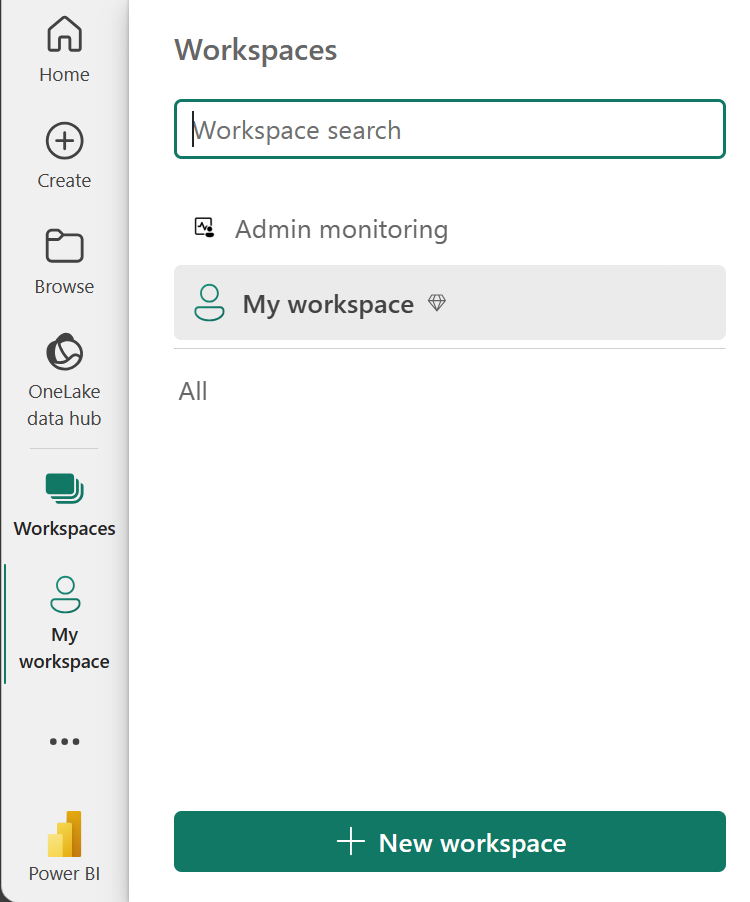
\includegraphics[scale=0.5]{images/01.png}\\
          Figura \thefigcount. Workspaces en Power BI.
          \stepcounter{figcount}
        \end{center}
    \end{minipage}

    Si aún no ha creado un informe, Power BI ofrece varios informes de ejemplo para explorar. Estos informes se cargan en Mi área de trabajo para que pueda explorar de forma privada. Puede acceder a informes de ejemplo en la sección Learn del panel de navegación.

    \begin{minipage}{\textwidth}
      \begin{center}
          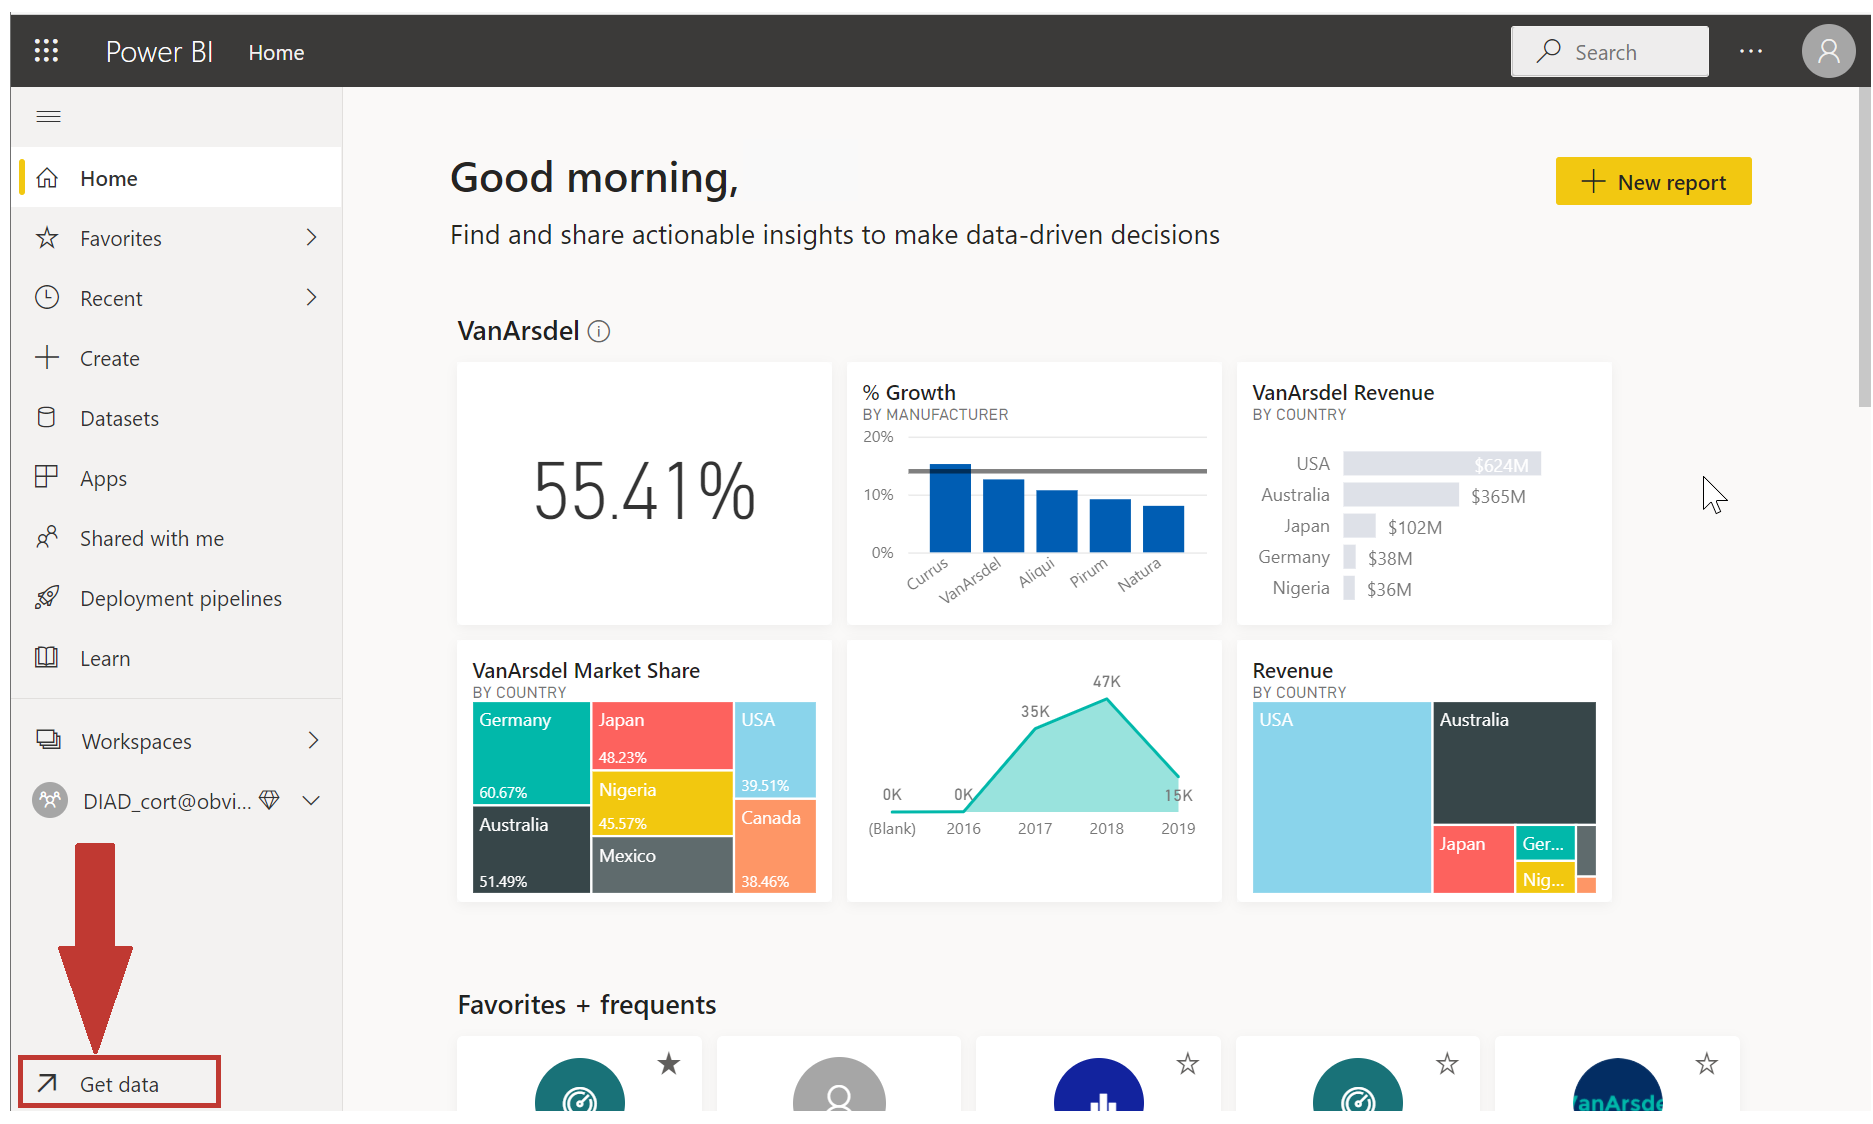
\includegraphics[scale=0.5]{images/02.png}\\
          Figura \thefigcount. Informes de ejemplo de Power BI.
          \stepcounter{figcount}
        \end{center}
    \end{minipage}

    En un área de trabajo, puede crear una aplicación, que proporciona a los consumidores una interfaz simplificada para acceder a informes y paneles. En la configuración de la aplicación, configura la aplicación, selecciona el contenido que se va a incluir (limitado al área de trabajo actual) y elige la audiencia.

    Una vez creada una aplicación, debe actualizar la aplicación después de cada cambio en los elementos del área de trabajo. El requisito de actualizar la aplicación permite controlar qué versión del contenido es visible para la audiencia.

    Captura de pantalla del centro de aprendizaje del servicio Power BI con informes de muestra incorporados.

    Las aplicaciones son la solución ideal para compartir dentro de cualquier organización. Aunque puede conceder acceso al área de trabajo, los permisos del área de trabajo pueden conceder a los usuarios acceso a más contenido del deseado. El uso compartido de elementos individuales también presenta un problema si realiza cambios que aún no desea que los consumidores vean.

\end{document}

\begin{minipage}{\textwidth}
  \begin{center}
      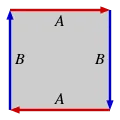
\includegraphics[scale=0.5]{images}\\
      Figura \thefigcount. Caption.
      \stepcounter{figcount}
    \end{center}
\end{minipage}